\documentclass[12pt,a4paper]{article}

% Margins.
\setlength{\oddsidemargin}{0in}
\setlength{\evensidemargin}{0in}
\setlength{\headheight}{12pt}
\setlength{\headsep}{0pt}
\setlength{\topmargin}{-60pt}
\setlength{\textwidth}{6.5in}
\setlength{\textheight}{10.75in}

\usepackage{amsmath}
\usepackage{float}
\usepackage{array}
\usepackage{graphicx}
\usepackage[hyphens]{url}
\usepackage{hyperref}	% Clickable links to figures, references and urls.
\usepackage{datetime}

% Drawing.
\usepackage{pgf}
\usepackage{tikz}

% Listings for formatting code.
\usepackage{listings}
\usepackage{textcomp}
% General options.
\lstset{breaklines=true, basicstyle=\small\ttfamily, tabsize=4, numbers=left, stepnumber=1, frame=single, showstringspaces=false, upquote=true}
% C++ specific high-lighting. Comments are 50/50 shades of green/black and strings coloured with 60/40 red/black mixture.
\lstset{language=[ISO]C++, commentstyle=\color{green!50!black}, keywordstyle=\color{blue}, stringstyle=\color{red!60!black}}

% Table cell alignment directives.
\newcolumntype{L}[1]{>{\raggedright\let\newline\\\arraybackslash\hspace{0pt}}m{#1}}
\newcolumntype{C}[1]{>{\centering\let\newline\\\arraybackslash\hspace{0pt}}m{#1}}
\newcolumntype{R}[1]{>{\raggedleft\let\newline\\\arraybackslash\hspace{0pt}}m{#1}}

%opening
\title{Data Structures and Algorithms\\Assignment 06\\Graphs}
\author{Attique Dawood}
\date{May 06, 2015\\Due: May 12, 2015\\[0.2cm] Last Modified: \today, \currenttime}
\begin{document}
\maketitle
\section{Task 1: Dijkstra's Algorithm}
Use the provided Dijkstra's algorithm code and apply it on following graph. Display shortest paths and distances in the form of a table from all source nodes. Repeat this assuming graph is undirected.
\begin{center}
\begin{tikzpicture}[->,>=stealth,shorten >=1pt,auto,node distance=3cm,
  thick,main node/.style={circle,fill=blue!10,draw,font=\sffamily\Large\bfseries}]

\node[main node] (a) {a};
\node[main node] (b) [below left of=a] {b};
\node[main node] (c) [below right of=b] {c};
\node[main node] (d) [below right of=a] {d};
\node[main node] (h) [right of=d] {h};
\node[main node] (e) [above right of =h] {e};
\node[main node] (f) [below right of=e] {f};
\node[main node] (g) [below left of=f] {g};

\path[every node/.style={font=\sffamily\small}]
	(d) edge node [left] {6} (a)
    (b) edge node [above] {2} (d)
	(a) edge node [above] {3} (e)
	(b) edge node [right] {4} (a)
	(c) edge node [right] {8} (b)
    (c) edge node [left] {3} (d)
	(d) edge node [above] {7} (h)
	(e) edge node [left] {5} (f)
	(e) edge node [right] {1} (h)
	(f) edge node [above] {2} (h)
	(f) edge node [left] {10} (g)
	(h) edge node [right] {3} (g)
	(g) edge node [above] {1} (c);
		
\end{tikzpicture}\\[0.2cm]
\end{center}
\section{Task 2: Directed Depth--First Search}
Implement directed depth--first search algorithm and apply it on following graph.
\begin{center}
\begin{tikzpicture}[->,>=stealth,shorten >=1pt,auto,node distance=3cm,
  thick,main node/.style={circle,fill=blue!10,draw,font=\sffamily\Large\bfseries}]

\node[main node] (1) {1};
\node[main node] (2) [below left of=1] {2};
\node[main node] (3) [below right of=2] {3};
\node[main node] (4) [below right of=1] {4};
\node[main node] (0) [above right of=4] {0};
\node[main node] (8) [below right of=0] {8};
\node[main node] (5) [above right of =8] {5};
\node[main node] (6) [below right of=5] {6};
\node[main node] (7) [below left of=6] {7};
\node[main node] (9) [below left of=8] {9};


\path[every node/.style={font=\sffamily\small}]
	(4) edge node [left] {} (1)
    (1) edge node [left] {} (3)
	(5) edge node [above] {} (0)
	(2) edge node [right] {} (1)
	(3) edge node [right] {} (2)
    (3) edge node [left] {} (4)
	(8) edge node [above] {} (4)
	(5) edge node [left] {} (6)
	(5) edge node [right] {} (8)
	(6) edge node [above] {} (8)
	(6) edge node [left] {} (7)
	(8) edge node [right] {} (0)
	(1) edge node [right] {} (0)
	(0) edge node [right] {} (4)
	(8) edge node [right] {} (9)
	(7) edge node [right] {} (9)
	(4) edge node [right] {} (9)
	(9) edge node [right] {} (3)
	(7) edge node [above] {} (8);
		
\end{tikzpicture}
\end{center}
\section{Task 3: Undirected Breadth--First Search}
Implement undirected breadth--first search algorithm and apply it on the graph given in task 2 assuming it is undirected.
\section{Implementation and Submission Guidelines}
It is strongly recommended that you make good use of STL containers as demonstrated in the given code; For example, using vector based adjacency list for storing graph. Submit Visual Studio 2010 \verb|.sln| and project files along with code files.
\end{document}
